% !TeX root = ../thesis.tex

\section{\acf{UEFI}}

It was designed to replace the legacy \acl{BF} \ac{BIOS} \TODO{which wasnt very standardized}, while also providing backwards compatibility by defining the \acf{CSM} allowing \ac{UEFI} firmware to boot legacy \ac{BIOS} applications.

boot- and runttime service functions for the bootloader and os to call
datatables containing platform-related information
% what are its concrete goals
- complete solution describing all features and capabilities
- abstract interfaces to support a range of processors without the need for knowledge about underlying hardware for the bootloader
- sharable persistent storage for platform support code
security


\subsection{\acs{UEFI} Images}

% https://edk2-docs.gitbook.io/edk-ii-build-specification/2_design_discussion/22_uefipi_firmware_images

files containing executable code
subset of PE32+ file format with modified header signature to distinguish from normal PE32 Images
+ stands for addition of 64-bit relocation fix-up extension

relocatable
fixed and dynamic address loading
loaded fully into memory and reloaction fix ups

three different subsystems types: application, boot service driver and runtime service driver
boot and runtime memory

application vs os loader vs driver
memory they reside in
unloaded on return
unloaded on error

memory marked as code and data
jump to entry point

\subsubsection{\acs{UEFI} Applications}

% https://edk2-docs.gitbook.io/edk-ii-uefi-driver-writer-s-guide/3_foundation/readme.7/371_applications

example efi shell
loaded by boot manager or other applications
return or calling exit specifically
always unloaded from memory

\subsubsection{UEFI OS Loaders}

% https://edk2-docs.gitbook.io/edk-ii-uefi-driver-writer-s-guide/3_foundation/readme.7/371_applications

example windows boot manager
normally take over control from the firmware
upon load behaves like a normal UEFI application
- only use memory allocated from the firmware
- only use services/protocols to access devices that the firmware exposes
- conform to driver specifications to access hardware
on error can return allocated resources with Exit boot service with error specific information given in ExitData
on success take full control with ExitBootServices boot service
all boot services in the system are terminated, including memory management
UEFI OS loader now responsible

\subsubsection{UEFI Drivers}

% https://edk2-docs.gitbook.io/edk-ii-uefi-driver-writer-s-guide/3_foundation/readme.7/372_drivers

loaded by boot manager, UEFI firmware (DXE foundation), or other applications
example payload
unloaded only when returning error code
presistent on success
boot and runtime drivers
only difference is that runtime are available after ExitBootServices was called
boottime drivers are terminated and memory is released
runttime drivers are fixed up with virtual mappings upon SetVirtualAddressMap call
has to convert its allocated memory

\subsection{\ac{UEFI} Driver Model}


\subsection{Protocols and Handles}
% https://edk2-docs.gitbook.io/edk-ii-uefi-driver-writer-s-guide/3_foundation/36_protocols_and_handles
% https://edk2-docs.gitbook.io/edk-ii-uefi-driver-writer-s-guide/3_foundation/34_handle_database
\cite[7.3 Protocol Handler Services]{uefi-spec}

% https://edk2-docs.gitbook.io/edk-ii-uefi-driver-writer-s-guide/3_foundation/35_guids
consists of GUID and protocol interface structure containing functions and instance data used to access a device

provide software abstractions for devices such as consoles, mass storage devices and networks
They can also be used to extend the number of generic services that are available in the platform
\cite[2.4 Protocols]{uefi-spec}
boot services provide function to install, locate, open, close and monitor protocols
\cite[7.3 Protocol Handler Services]{uefi-spec}
% https://edk2-docs.gitbook.io/edk-ii-uefi-driver-writer-s-guide/5_uefi_services/51_services_that_uefi_drivers_commonly_use/513_handle_database_and_protocol_services
identified with guids
\subsection{Variables}
key/value pairs
store arbirtary data passed between UEFI environment and applications/os loaders
type of data is defined through usage
storage implementation is not specify but must support non volatility if demanded to be able to be retained after reboots
variables are defined by their Vendor GUID, Name and attributes such as: their scope (boot time, run time, non-volatile), whether writes require authentication or result in appending data instead of overriding
\cite[8.2]{uefi-spec}
\TODO{deep dive in authenticated variables}
architecually defined variables are called Globally Defined Variables where vendor GUID is defined with the macro \lstinline{EFI_GLOBAL_VARIABLE}
\cite[3.3]{uefi-spec}
relevant for secure boot and boot manager

\subsection{Systemtable}
% https://edk2-docs.gitbook.io/edk-ii-uefi-driver-writer-s-guide/3_foundation/33_uefi_system_table
system tables offers boot and runtime services
supplied by drivers implementing arichtectural protocols % how to uefi buch zitat
\subsubsection{Boottime Services}
\subsubsection{Runtime Services}

\subsection{\acf{GPT}}
\ac{MBR} boot code, four partitions
\ac{GUID} for uniquely identifying each partition
\ac{GUID} for partition type content
\ac{GPT}
\ac{LBA}
legacy \ac{MBR} or protective \ac{MBR}


\cite[5]{uefi-spec}
\subsection{\acf{ESP}}
\ac{FAT}32 \cite[13.3]{uefi-spec}
can reside on any media that is supported by EFI Boot Services
\cite[13.3.1]{uefi-spec}

\subsection{Boot Manager}

\autoref{fig:uefi-boot-sequence}

what is the boot manager
which drivers and applications and when
firmware policy engine
configured by non volatile variables
\cite[3.1.]{uefi-spec}
boot manager = bds
boot behavior
\subsubsection{Boot Variables}
boot options variables
boot options (network, simple file system protocol, load file)
default boot behavior for simple file system protocol

EFI boot variable must contain a short description of the boot entry, the complete
device and file path of the Boot Manager, and some optional data
\cite{windows-internals-7-part2}

\begin{figure}[htb]%
    \centering%
    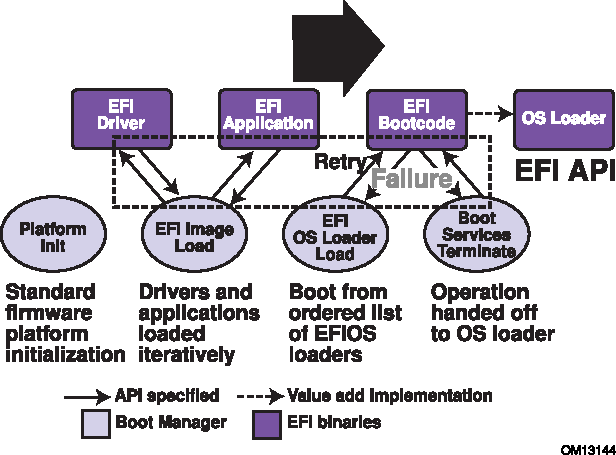
\includegraphics[width=\textwidth]{uefi_boot_sequence}%
    \caption{Booting Sequence \cite[Figure 2-1]{uefi-spec}}%
    \label{fig:uefi-boot-sequence}%
\end{figure}